%#########################1########################

\stepcounter{section}
\begin{center}
	\textbf{\color{color2} \thesection} \quad  \textbf{Integración del presupuesto en SAN del plan del pacto Hambre Cero a nivel nacional} \addcontentsline{toc}{section}{\numberline{\thesection} Integración del presupuesto en SAN del plan del pacto Hambre Cero a nivel nacional}
\end{center}
$\ $ \\[-5cm]
 \cajita{%
Tasa de Asignación presupuestaria en Seguridad Alimentaria y Nutricional (SAN), del Pacto Hambre Cero (PH0) años 2012 a 2015 }%
{%
	Hambre Cero es un programa social del Gobierno guatemalteco introducido  en 2012 con el objetivo de erradicar la desnutrición crónica infantil y la pobreza extrema.
	
	El Pacto Hambre Cero, busca disminuir en 10\% la prevalencia de la desnutrición crónica en un plazo de 4 años, lo cual será la base para lograr una reducción del 24\% en los próximos 10 años.  En 2015 la tasa de asignación respecto del presupuesto general de la nación fue de 7.7 \%.  
 }%
{%
Tasa de Asignación presupuestaria en Seguridad Alimentaria y Nutricional (SAN), del Pacto Hambre Cero (PH0) respecto del presupuesto general de la nación } %
{%
 República de Guatemala, serie histórica, en porcentaje} %
{%
 \begin{tikzpicture}[x=1pt,y=1pt]  \input{graficas/7_01.tex}  \end{tikzpicture}}%
{%
 Sicoin} %


 \cajita{%
 	Ejecución presupuestaria en Seguridad Alimentaria y Nutricional (SAN), del Pacto Hambre Cero (PH0)}%
 {%
 	
 	
 	La ejecución presupuestaria en Seguridad Alimentaria y Nutricional (SAN), del Pacto Hambre Cero (PH0) entre el 2012 y 2015 ha variado entre 66.6 y 89.2 por ciento, teniendo su ejecuación más baja en el 2015.
 }%
 {%
 	Tasa de ejecución de la Sesan respecto al presupuesto asignado } %
 {%
 	República de Guatemala, serie histórica, en porcentaje} %
 {%
 	\begin{tikzpicture}[x=1pt,y=1pt]  \input{graficas/7_02.tex}  \end{tikzpicture}}%
 {%
 	Sicoin} %
 
 
  \cajita{%
  	Detalle de presupuesto asignado del plan del Pacto Hambre Cero (PPH0) }%
  {%
  	Para atender la desnutrición se implementó el plan hambre cero, siendo la Sesan parte importante en la ejecución del mismo. 
  		
  		En Plan Hambre Cero está compuesto por componentes directos, de viabilidad y el eje transversal, siendo este último el aspecto en el que menos se invirtió dinero por parte del estado para el 2015.
  }%
  {%
  	Detalle de ejecución para el plan del Pacto Hambre Cero (PPH0) } %
  {%
  	República de Guatemala, 2015, en quetzales} %
  {%
  	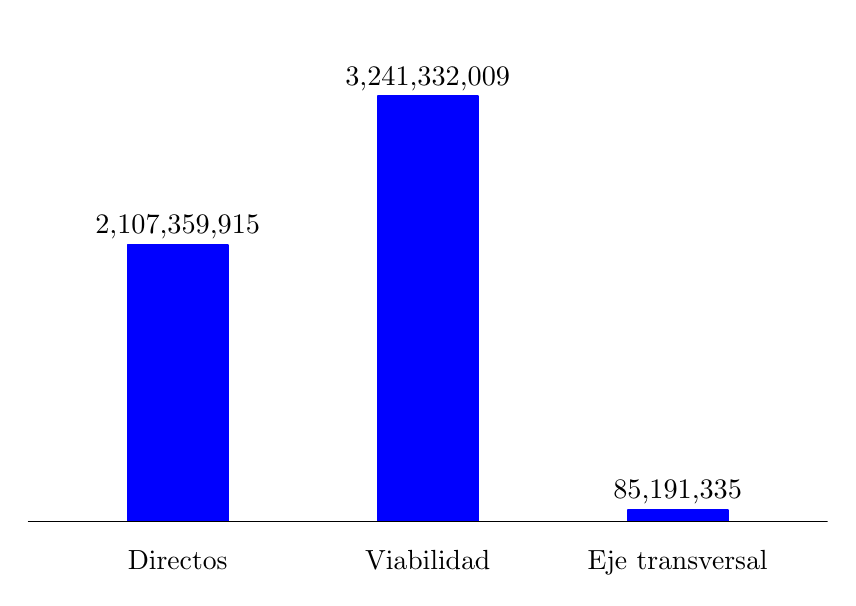
\begin{tikzpicture}[x=1pt,y=1pt]  % Created by tikzDevice version 0.9 on 2016-03-03 06:36:59
% !TEX encoding = UTF-8 Unicode
\definecolor{fillColor}{RGB}{255,255,255}
\path[use as bounding box,fill=fillColor,fill opacity=0.00] (0,0) rectangle (289.08,198.74);
\begin{scope}
\path[clip] (  0.00,  0.00) rectangle (289.08,198.74);

\path[] (  0.00,  0.00) rectangle (289.08,198.74);
\end{scope}
\begin{scope}
\path[clip] (  0.00,  0.00) rectangle (289.08,198.74);

\path[] (  0.00, 12.77) rectangle (289.08,181.67);

\path[] ( 54.20, 12.77) --
	( 54.20,181.67);

\path[] (144.54, 12.77) --
	(144.54,181.67);

\path[] (234.88, 12.77) --
	(234.88,181.67);
\definecolor{drawColor}{RGB}{0,0,255}
\definecolor{fillColor}{RGB}{0,0,255}

\path[draw=drawColor,line width= 0.6pt,line join=round,fill=fillColor] ( 36.13, 20.44) rectangle ( 72.27,120.27);

\path[draw=drawColor,line width= 0.6pt,line join=round,fill=fillColor] (126.47, 20.44) rectangle (162.61,173.99);

\path[draw=drawColor,line width= 0.6pt,line join=round,fill=fillColor] (216.81, 20.44) rectangle (252.95, 24.48);
\definecolor{drawColor}{RGB}{0,0,0}

\path[draw=drawColor,line width= 0.1pt,line join=round] (  0.00, 20.44) -- (289.08, 20.44);

\node[text=drawColor,anchor=base,inner sep=0pt, outer sep=0pt, scale=  1.02] at ( 54.20,124.25) {2,107,359,915};

\node[text=drawColor,anchor=base,inner sep=0pt, outer sep=0pt, scale=  1.02] at (144.54,177.96) {3,241,332,009};

\node[text=drawColor,anchor=base,inner sep=0pt, outer sep=0pt, scale=  1.02] at (234.88, 28.45) {85,191,335};

\path[] (  0.00, 12.77) rectangle (289.08,181.67);
\end{scope}
\begin{scope}
\path[clip] (  0.00,  0.00) rectangle (289.08,198.74);

\path[] (  0.00, 12.77) --
	(289.08, 12.77);
\end{scope}
\begin{scope}
\path[clip] (  0.00,  0.00) rectangle (289.08,198.74);

\path[] ( 54.20, 10.02) --
	( 54.20, 12.77);

\path[] (144.54, 10.02) --
	(144.54, 12.77);

\path[] (234.88, 10.02) --
	(234.88, 12.77);
\end{scope}
\begin{scope}
\path[clip] (  0.00,  0.00) rectangle (289.08,198.74);
\definecolor{drawColor}{RGB}{0,0,0}

\node[text=drawColor,anchor=base,inner sep=0pt, outer sep=0pt, scale=  1.00] at ( 54.20, 3.00) {Directos};

\node[text=drawColor,anchor=base,inner sep=0pt, outer sep=0pt, scale=  1.00] at (144.54, 3.00) {Viabilidad};

\node[text=drawColor,anchor=base,inner sep=0pt, outer sep=0pt, scale=  1.00] at (234.88, 3.00) {Eje transversal};
\end{scope}
  \end{tikzpicture}}%
  {%
  	Sicoin} %
  
  
  
  \cajita{%
  	Asignación presupuestaria a la Ventana de los Mil Días}%
  {%	
  	En la serie histórica se observa que ha habido un aumento en la inversión para el Plan la Ventana de los Mil Días. En el 2015 se hizo una asignación de 705,840,558 quetzales. 
  }%
  {%
  Asignación presupuestaria al programa ventana de los mi días para el año 2015} %
  {%
  	República de Guatemala, serie histórica, en quetzales} %
  {%
  	\begin{tikzpicture}[x=1pt,y=1pt]  \input{graficas/7_04.tex}  \end{tikzpicture}}%
  {%
  	Sicoin} %
  
  
    \cajita{%
    	Gasto Programa Ventana de los Mil Días}%
    {%
    	El Programa  Ventana de los Mil Días tiene varios rubros de inversión.
    	
    	Para el 2015 el gasto se centralizó en la compra de vacunas, seguido de la compra de Vitamina A.
    }%
    {%
    	Detalle del gasto en el Plan Ventana de los Mil Días} %
    {%
    	República de Guatemala, 2015, en miles de millones quetzales} %
    {%
    	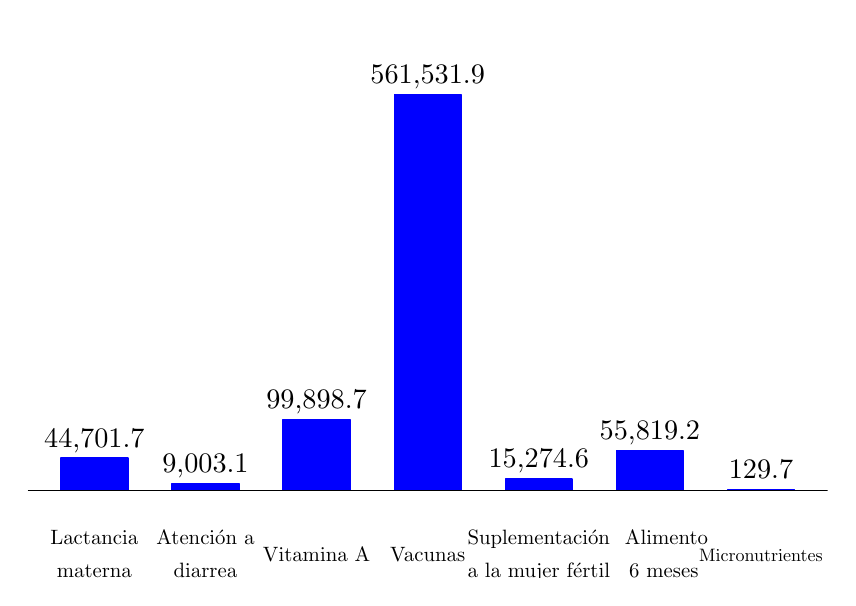
\begin{tikzpicture}[x=1pt,y=1pt]  % Created by tikzDevice version 0.9 on 2016-03-03 06:46:08
% !TEX encoding = UTF-8 Unicode
\definecolor{fillColor}{RGB}{255,255,255}
\path[use as bounding box,fill=fillColor,fill opacity=0.00] (0,0) rectangle (289.08,198.74);
\begin{scope}
\path[clip] (  0.00,  0.00) rectangle (289.08,198.74);

\path[] (  0.00,  0.00) rectangle (289.08,198.74);
\end{scope}
\begin{scope}
\path[clip] (  0.00,  0.00) rectangle (289.08,198.74);

\path[] (  0.00, 24.65) rectangle (289.08,181.67);

\path[] ( 24.09, 24.65) --
	( 24.09,181.67);

\path[] ( 64.24, 24.65) --
	( 64.24,181.67);

\path[] (104.39, 24.65) --
	(104.39,181.67);

\path[] (144.54, 24.65) --
	(144.54,181.67);

\path[] (184.69, 24.65) --
	(184.69,181.67);

\path[] (224.84, 24.65) --
	(224.84,181.67);

\path[] (264.99, 24.65) --
	(264.99,181.67);
\definecolor{drawColor}{RGB}{0,0,255}
\definecolor{fillColor}{RGB}{0,0,255}

\path[draw=drawColor,line width= 0.6pt,line join=round,fill=fillColor] ( 12.04, 31.78) rectangle ( 36.14, 43.15);

\path[draw=drawColor,line width= 0.6pt,line join=round,fill=fillColor] ( 52.20, 31.78) rectangle ( 76.29, 34.07);

\path[draw=drawColor,line width= 0.6pt,line join=round,fill=fillColor] ( 92.35, 31.78) rectangle (116.43, 57.18);

\path[draw=drawColor,line width= 0.6pt,line join=round,fill=fillColor] (132.50, 31.78) rectangle (156.59,174.53);

\path[draw=drawColor,line width= 0.6pt,line join=round,fill=fillColor] (172.64, 31.78) rectangle (196.73, 35.67);

\path[draw=drawColor,line width= 0.6pt,line join=round,fill=fillColor] (212.80, 31.78) rectangle (236.88, 45.97);

\path[draw=drawColor,line width= 0.6pt,line join=round,fill=fillColor] (252.94, 31.78) rectangle (277.03, 31.82);
\definecolor{drawColor}{RGB}{0,0,0}

\path[draw=drawColor,line width= 0.1pt,line join=round] (  0.00, 31.78) -- (289.08, 31.78);

\node[text=drawColor,anchor=base,inner sep=0pt, outer sep=0pt, scale=  1.02] at ( 24.09, 47.12) {44,701.7};

\node[text=drawColor,anchor=base,inner sep=0pt, outer sep=0pt, scale=  1.02] at ( 64.24, 38.04) {9,003.1};

\node[text=drawColor,anchor=base,inner sep=0pt, outer sep=0pt, scale=  1.02] at (104.39, 61.15) {99,898.7};

\node[text=drawColor,anchor=base,inner sep=0pt, outer sep=0pt, scale=  1.02] at (144.54,178.50) {561,531.9};

\node[text=drawColor,anchor=base,inner sep=0pt, outer sep=0pt, scale=  1.02] at (184.69, 39.64) {15,274.6};

\node[text=drawColor,anchor=base,inner sep=0pt, outer sep=0pt, scale=  1.02] at (224.84, 49.95) {55,819.2};

\node[text=drawColor,anchor=base,inner sep=0pt, outer sep=0pt, scale=  1.02] at (264.99, 35.79) {129.7};

\path[] (  0.00, 24.65) rectangle (289.08,181.67);
\end{scope}
\begin{scope}
\path[clip] (  0.00,  0.00) rectangle (289.08,198.74);

\path[] (  0.00, 24.65) --
	(289.08, 24.65);
\end{scope}
\begin{scope}
\path[clip] (  0.00,  0.00) rectangle (289.08,198.74);

\path[] ( 24.09, 21.90) --
	( 24.09, 24.65);

\path[] ( 64.24, 21.90) --
	( 64.24, 24.65);

\path[] (104.39, 21.90) --
	(104.39, 24.65);

\path[] (144.54, 21.90) --
	(144.54, 24.65);

\path[] (184.69, 21.90) --
	(184.69, 24.65);

\path[] (224.84, 21.90) --
	(224.84, 24.65);

\path[] (264.99, 21.90) --
	(264.99, 24.65);
\end{scope}
\begin{scope}
\path[clip] (  0.00,  0.00) rectangle (289.08,198.74);
\definecolor{drawColor}{RGB}{0,0,0}

\node[text=drawColor,anchor=base,inner sep=0pt, outer sep=0pt, scale=  0.750] at ( 24.09, 11.88) {Lactancia };

\node[text=drawColor,anchor=base,inner sep=0pt, outer sep=0pt, scale=  0.750] at ( 24.09,  0.00) {  materna};

\node[text=drawColor,anchor=base,inner sep=0pt, outer sep=0pt, scale=  0.750] at ( 64.24, 11.88) {Atención a };

\node[text=drawColor,anchor=base,inner sep=0pt, outer sep=0pt, scale=  0.750] at ( 64.24,  0.00) { diarrea};

\node[text=drawColor,anchor=base,inner sep=0pt, outer sep=0pt, scale=  0.750] at (104.39,  5.94) {Vitamina A};

\node[text=drawColor,anchor=base,inner sep=0pt, outer sep=0pt, scale=  0.750] at (144.54,  5.94) {Vacunas};

\node[text=drawColor,anchor=base,inner sep=0pt, outer sep=0pt, scale=  0.750] at (184.69, 11.88) {Suplementación};

\node[text=drawColor,anchor=base,inner sep=0pt, outer sep=0pt, scale=  0.750] at (184.69,  0.00) {a la  mujer fértil};

\node[text=drawColor,anchor=base,inner sep=0pt, outer sep=0pt, scale=  0.750] at (230.84, 11.88) {Alimento};

\node[text=drawColor,anchor=base,inner sep=0pt, outer sep=0pt, scale=  0.750] at (229.84,  0.00) { 6 meses};

\node[text=drawColor,anchor=base,inner sep=0pt, outer sep=0pt, scale=  0.650] at (264.99,  5.94) {Micronutrientes};
\end{scope}
  \end{tikzpicture}}%
    {%
    	Sicoin} %
  